\chapter{Binarisierung}
\section{Binarisierung der Bilder}
Das Binarisieren der importierten Bilder stellt die erste Hürde im Binarisierungsprozess des \textit{NNs} auf. Wir arbeiten in unserem \textit{BNN} mit \textit{Grey-Scaled}-Bildern, d.h. wir verarbeiten nur einen $\alpha$\textit{-Kanal} anstatt drei \textit{RGB-Kanälen}. Dieser $\alpha$\textit{-Kanal} bewegt sich jedoch in einem Wertebereich von $\{0-255\}$ bzw. $(0,1)$ mit einer Granularität von $\frac{1}{255}$.\\

Unsere Aufgabe bei der Binarisierung ist es also mit möglichst wenig Informationsverlust eine Funktion $\mathbb{Q}_{0-1} \rightarrow \{0,1\}$ zu entwickeln, die unsere importierten Bilder binarisiert.

\subsection{Threshold}

Im Folgenden betrachten wir den Wertebereich der Pixel als zwischen $\{0-255\}$ liegend.\\Der erste Ansatz für eine Binarisierungsfunktion waren Thresholds. Diese Funktion flippt für ein fest gewähltes $n \in \{0..255\}$ alle Bits, die den Schwellenwert $n$ überschreiten, auf $1$ und alle anderen auf $0$.\\

Der Vorteil dieser Methode ist, dass man eine sehr kostengünstige Binarisierung erhält. Man kann durch das fest gewählte $n$ die \textit{Inbuild}-Tensor-Funktionen verwenden und muss nicht manuell über die einzelnen Pixel iterieren. Dies ist vorallem wichtig, da man mit $30.000$ Bildern je $28 \times 28$ Pixeln sehr viele Binarisierungsschritte erhält.\\

Der große Nachteil an der Threshold-Methode ist, dass man kompromisse machen muss. Es gibt nicht einen guten Threshhold, da für jeden gewählten Threshold bei einer Teilmenge der Bilder zuviel, bzw. zu wenig gefiltert wird. (Siehe Abbildung 5.1 bzw. 5.2)
\begin{figure}[h]
\centering
\begin{minipage}{.5\textwidth}
  \centering
  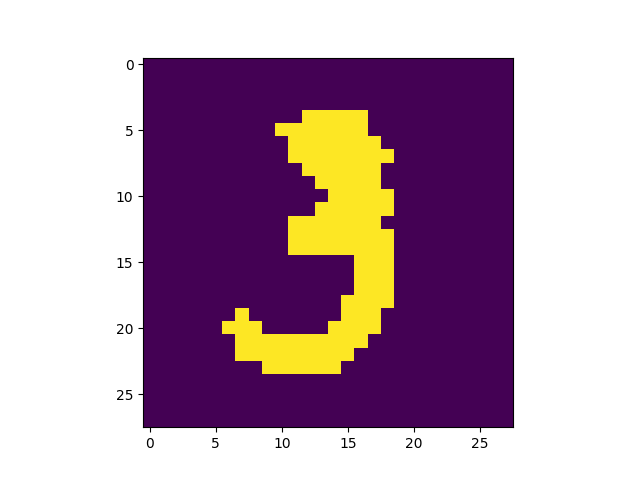
\includegraphics[width=.4\linewidth]{./bilder/comparison/threshold/100_3}
  \captionof{figure}{3, Threshold 100}
  \label{fig:bin3}
\end{minipage}%
\begin{minipage}{.5\textwidth}
  \centering
  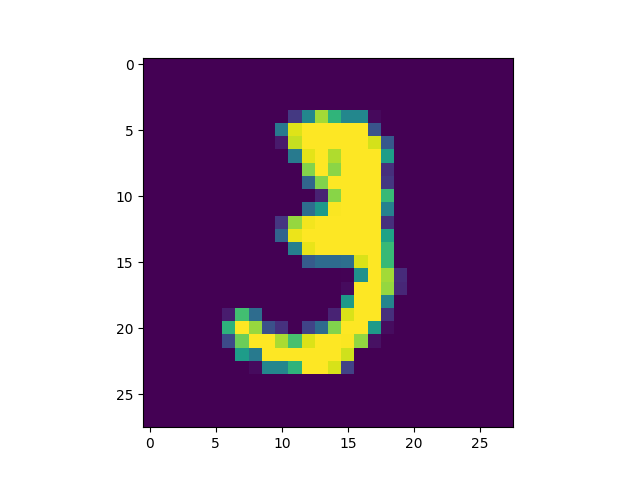
\includegraphics[width=.4\linewidth]{./bilder/comparison/default_3}
  \captionof{figure}{3, not binarized}
  \label{fig:dflt}
\end{minipage}
\begin{minipage}{.5\textwidth}
  \centering
  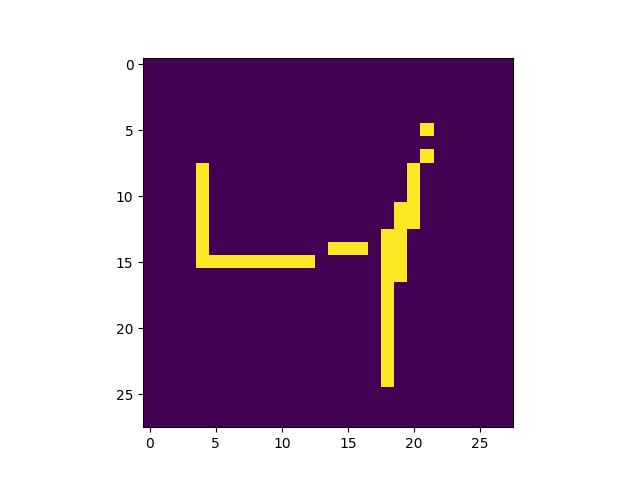
\includegraphics[width=.4\linewidth]{./bilder/comparison/threshold/200}
  \captionof{figure}{4, Threshold 200}
  \label{fig:bin4}
\end{minipage}%
\begin{minipage}{.5\textwidth}
  \centering
  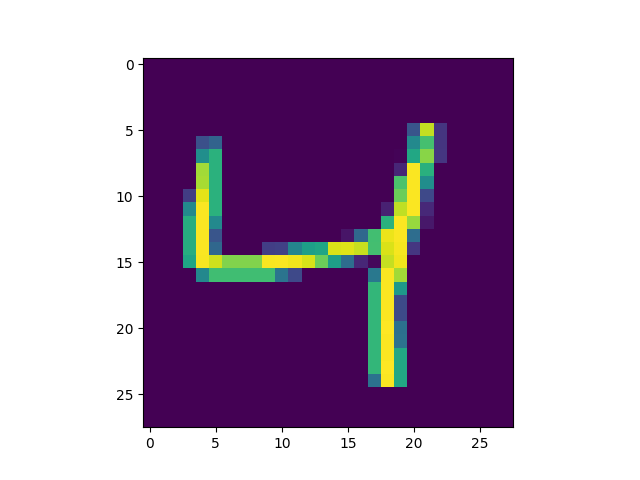
\includegraphics[width=.4\linewidth]{./bilder/comparison/default}
  \captionof{figure}{4, not binarized}
  \label{fig:dflt}
\end{minipage}

\end{figure}
In diesem Vergleich sieht man sehr gut, dass ein Threshold, der für ein Bild zu tief gesetzt ist, d.h. es werden zu wenig Pixel gefiltert nicht erhöht werden kann, da er sonst für ein anderes Bild zu hoch gesetzt ist(es werden zu viele Pixel gefiltert).\\

\subsection{Probability}

Eine Lösung für dieses Problem bietet die \textit{Probability-Transformation}. Bei dieser Methode betrachten wir den Wert eines einzelnen Pixels als die Warscheinlichkeit, dass dieser Pixel in der Binarisierung mit $1$ belegt wird.\\

Nachteil dieser Methode ist die Effizienz. Da wir nun nicht mehr mit einem statischen Threshold arbeiten, müssen wir manuell über die Pixel iterieren. Dabei verschlechtern wir uns im Zeitlichen um einen Faktor $20$. Somit ist das Trainieren mit der \textit{Probability-Transformation} deutlich teurer. Einen wichtigen Geschwindigkeitsboost hat die Umwandlung des Pixeltensors in einen \textit{Numpy-Array} gegeben. Diesen zu bearbeiten ist $~6$ mal effizienter als einen Tensor zu bearbeiten.\\

Der große Vorteil dieser Methode ist jedoch die Informationserhaltung. Wir arbeiten bei der \textit{Probability-Transformation} mit sogenannten \textit{Repetitions}. Diese durchlaufen die gleiche Generation mit dem gleichen \textit{Trainingset}, welche jedoch neu binarisiert wurden. Das heißt, dass man bei 50 Repetitions jede Generation 50 mal, mit 50 unabhängig binarisierten \textit{Trainginsets} durchläuft.\\Dadurch erhalten wir ein Mittel für jedes Bild, welches gegen die Originalversion konvergiert. (Siehe Abbildung 5.5 bzw 5.6)

\begin{figure}[h]
\centering
\begin{minipage}{.5\textwidth}
  \centering
  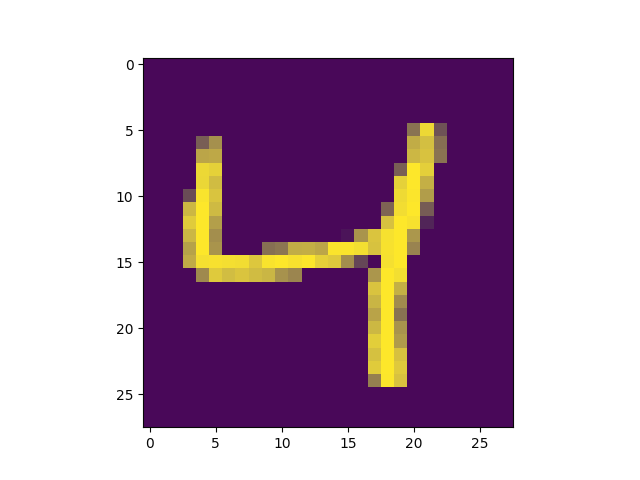
\includegraphics[width=.4\linewidth]{./bilder/comparison/overlapped}
  \captionof{figure}{4, overlapped 50 prob-trans}
  \label{fig:bin3}
\end{minipage}%
\begin{minipage}{.5\textwidth}
  \centering
  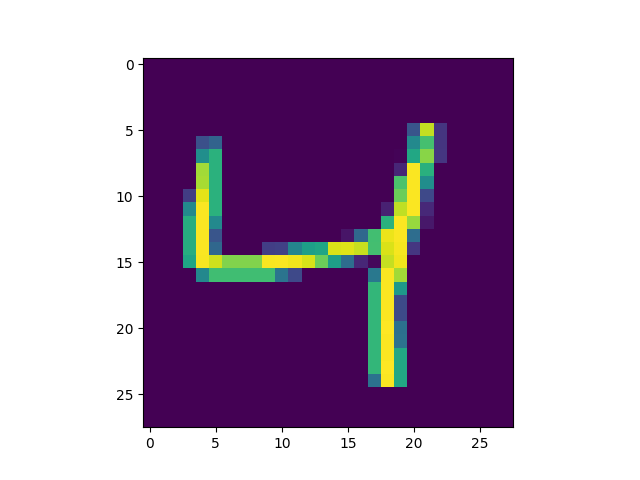
\includegraphics[width=.4\linewidth]{./bilder/comparison/default}
  \captionof{figure}{4, not binarized}
  \label{fig:dflt}
\end{minipage}
\end{figure}

Somit konvergiert auch die Genauigkeit zu der Genauigkeit ohne \textit{Input-Binarization} auf Kosten der Laufzeit.\\Die einzelnen Bilder, aus denen sich Abbildung 5.5 zusammensetzt finden sich im Anhang.


